\documentclass[12pt,a4paper]{article}
\usepackage[utf8]{inputenc}
\usepackage[spanish]{babel}
\usepackage[margin=2.5cm]{geometry}
\usepackage{graphicx}
\graphicspath{{images/}}
\usepackage{booktabs}
\usepackage{longtable}
\usepackage{array}
\usepackage{hyperref}
\usepackage{xcolor}
\usepackage{titlesec}
\usepackage{fancyhdr}
\usepackage{enumitem}
\usepackage{tabularx}
\usepackage{float}

\definecolor{azulprimario}{HTML}{4A82C7}
\definecolor{grisoscuro}{HTML}{333333}
\definecolor{rojoadmin}{HTML}{C0392B}

\hypersetup{
    colorlinks=true,
    linkcolor=azulprimario,
    urlcolor=azulprimario,
    citecolor=azulprimario
}

\titleformat{\section}{\Large\bfseries\color{grisoscuro}}{}{0em}{}[\titlerule]
\titleformat{\subsection}{\large\bfseries\color{azulprimario}}{}{0em}{}

\pagestyle{fancy}
\fancyhf{}
\fancyhead[L]{\small\textcolor{gray}{NexaCommerce --- SRS v1.0}}
\fancyhead[R]{\small\textcolor{gray}{Jordan Guam\'an}}
\fancyfoot[C]{\thepage}
\renewcommand{\headrulewidth}{0.4pt}

\begin{document}

% ==================== PORTADA ====================
\begin{titlepage}
\centering
\vspace*{2cm}
{\Huge\bfseries Especificaci\'on de Requisitos de Software (SRS)\par}
\vspace{1cm}
{\LARGE\textcolor{azulprimario}{NexaCommerce}\par}
\vspace{0.5cm}
{\large Plataforma de E-Commerce basada en Microservicios\par}
\vspace{2cm}
\begin{tabular}{ll}
\textbf{Versi\'on:} & 1.0 \\
\textbf{Fecha:} & 24 de Febrero de 2026 \\
\textbf{Autor:} & Jordan Guam\'an \\
\textbf{Instituci\'on:} & Universidad de las Fuerzas Armadas -- ESPE \\
\textbf{Sede:} & Sangolqu\'i \\
\textbf{Per\'iodo:} & Marzo 2023 -- Julio 2023 \\
\end{tabular}
\vfill
{\small Documento elaborado siguiendo el est\'andar IEEE Std 830-1998}
\end{titlepage}

% ==================== INDICE ====================
\tableofcontents
\newpage

% ==================== 1. INTRODUCCION ====================
\section{Introducci\'on}

\subsection{Prop\'osito}
El presente documento define la Especificaci\'on de Requisitos de Software (SRS) para \textbf{NexaCommerce}, una plataforma de comercio electr\'onico construida sobre una arquitectura de microservicios. El objetivo es detallar los requisitos funcionales y no funcionales, los casos de uso, las restricciones t\'ecnicas y las decisiones de dise\~no que guiar\'an el desarrollo del sistema.

Este documento est\'a dirigido a:
\begin{itemize}
    \item Desarrolladores del equipo de backend y frontend
    \item Arquitectos de software
    \item Docentes evaluadores del proyecto
    \item Stakeholders interesados en la plataforma
\end{itemize}

\subsection{Alcance}
\textbf{NexaCommerce} es una plataforma web de comercio electr\'onico que permite a los usuarios registrarse, explorar un cat\'alogo de productos, gestionar un carrito de compras, realizar pedidos y consultar el historial de compras. Adicionalmente, los administradores pueden gestionar el inventario, procesar pedidos y consultar reportes de ventas.

El sistema se compone de:
\begin{itemize}
    \item \textbf{5 microservicios backend} independientes (Usuarios, Productos, Carrito, Pedidos, Reportes)
    \item \textbf{1 API Gateway} como punto de entrada unificado
    \item \textbf{1 aplicaci\'on frontend} SPA (Single Page Application)
    \item \textbf{2 bases de datos} (MongoDB para datos transaccionales, MySQL para reportes)
\end{itemize}

\subsection{Definiciones y Acr\'onimos}
\begin{table}[H]
\centering
\begin{tabular}{ll}
\toprule
\textbf{Acr\'onimo} & \textbf{Definici\'on} \\
\midrule
SRS & Software Requirements Specification \\
API & Application Programming Interface \\
JWT & JSON Web Token \\
SPA & Single Page Application \\
CRUD & Create, Read, Update, Delete \\
REST & Representational State Transfer \\
MS & Microservicio \\
RF & Requisito Funcional \\
RNF & Requisito No Funcional \\
\bottomrule
\end{tabular}
\end{table}

\subsection{Referencias}
\begin{itemize}
    \item IEEE Std 830-1998: Pr\'actica recomendada para SRS
    \item Documentaci\'on oficial de Node.js (\url{https://nodejs.org})
    \item Documentaci\'on oficial de Vue.js 3 (\url{https://vuejs.org})
    \item Documentaci\'on de MongoDB (\url{https://docs.mongodb.com})
    \item Documentaci\'on de Express.js (\url{https://expressjs.com})
\end{itemize}

\newpage
% ==================== 2. DESCRIPCION GENERAL ====================
\section{Descripci\'on General del Sistema}

\subsection{Perspectiva del Producto}
NexaCommerce es un sistema nuevo e independiente que demuestra la aplicaci\'on pr\'actica de la arquitectura de microservicios en un contexto de comercio electr\'onico. Cada microservicio opera de forma aut\'onoma con su propia base de datos, comunic\'andose entre s\'i mediante APIs REST.

% --- DIAGRAMA: ARQUITECTURA ---
\begin{figure}[H]
\centering
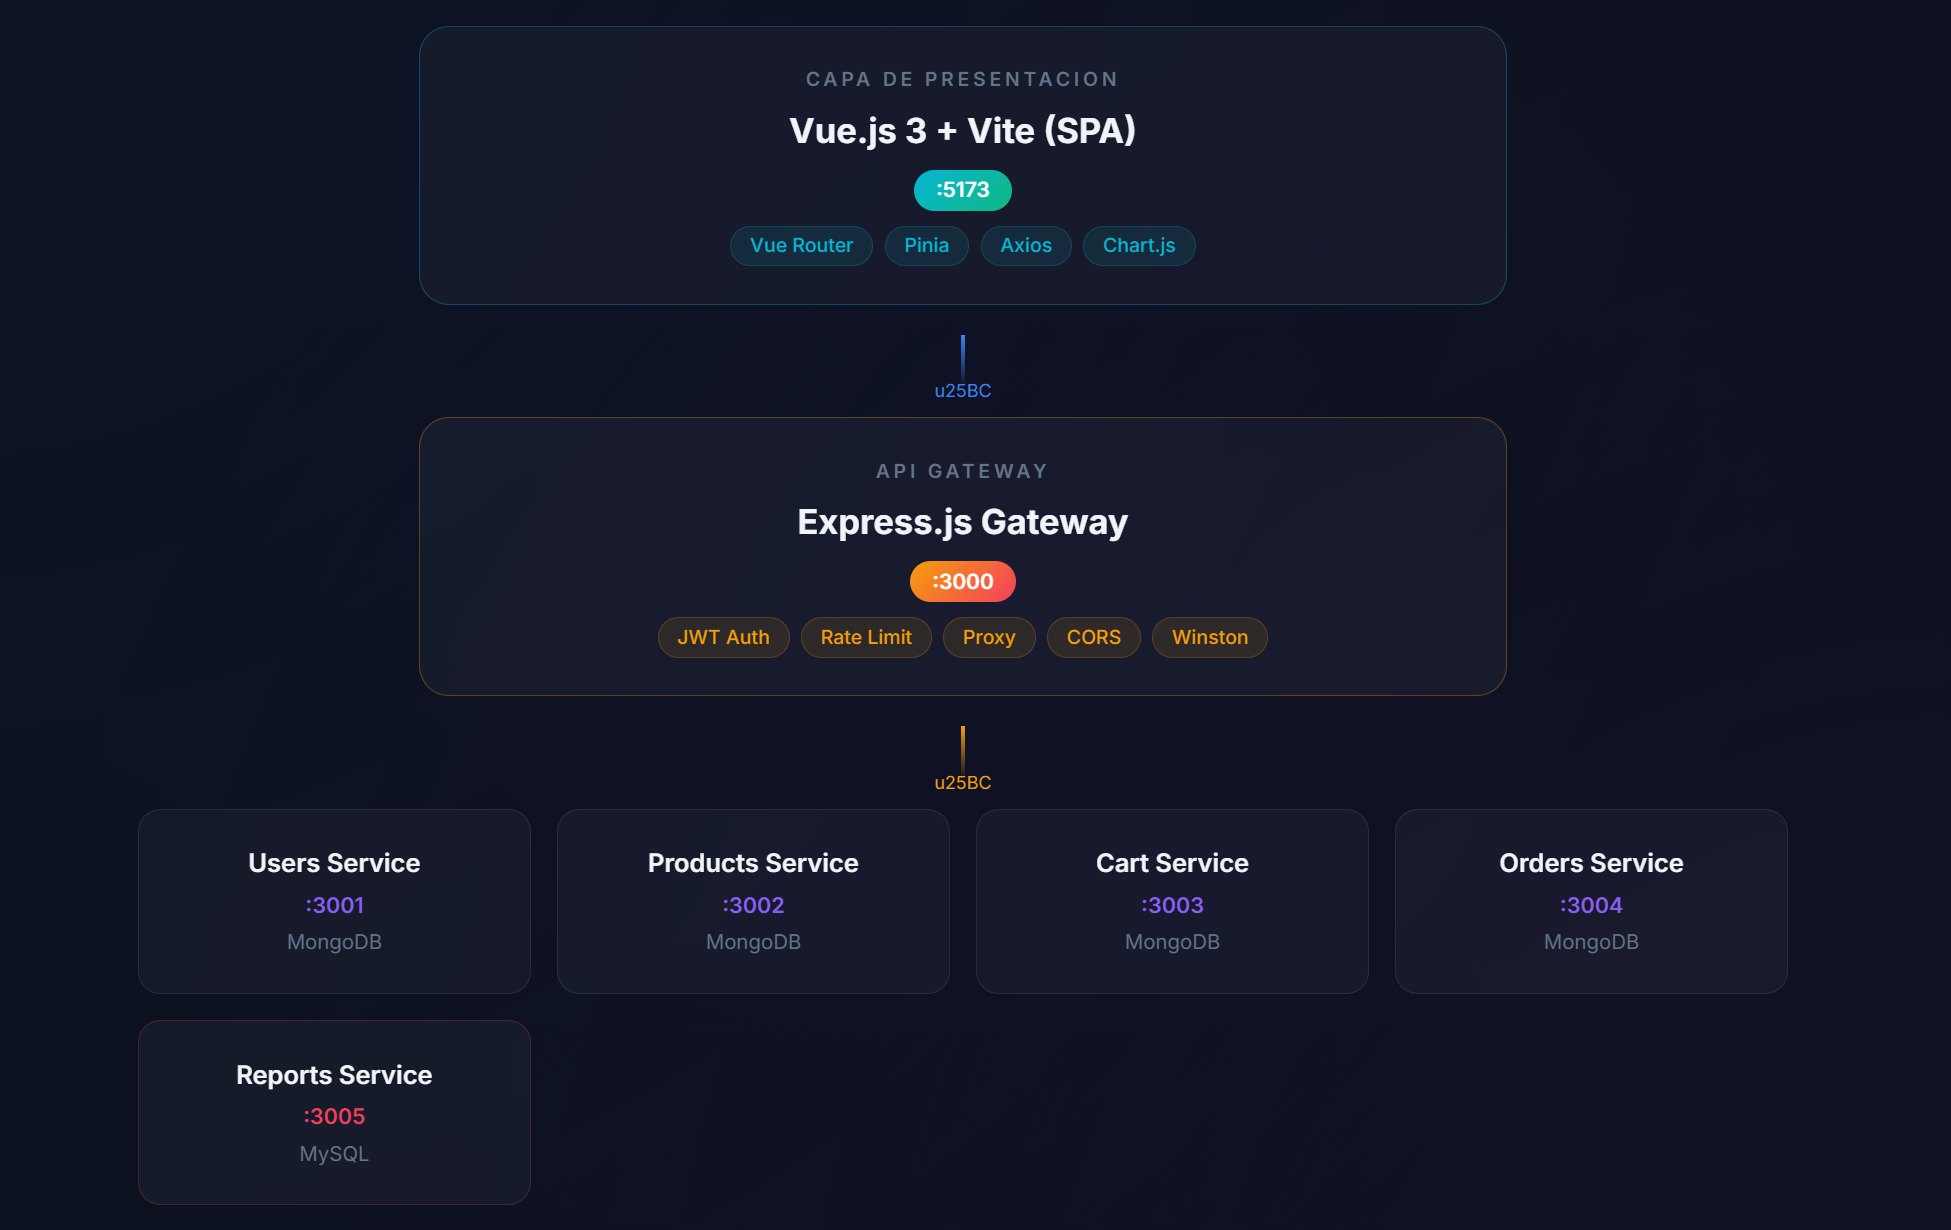
\includegraphics[width=0.85\textwidth]{diagrama_arquitectura.png}
\caption{Diagrama de Arquitectura de Microservicios de NexaCommerce}
\label{fig:arquitectura}
\end{figure}

\subsection{Funciones Principales del Producto}
\begin{table}[H]
\centering
\begin{tabularx}{\textwidth}{clX}
\toprule
\textbf{\#} & \textbf{Funci\'on} & \textbf{Descripci\'on} \\
\midrule
1 & Gesti\'on de Usuarios & Registro, autenticaci\'on, perfiles y roles \\
2 & Cat\'alogo de Productos & CRUD de productos con categor\'ias, b\'usqueda y filtros \\
3 & Carrito de Compras & Agregar, modificar y eliminar items del carrito \\
4 & Procesamiento de Pedidos & Crear pedidos, gestionar estados, historial \\
5 & Reportes y An\'alisis & Reportes de ventas, productos top, ingresos \\
6 & Panel de Administraci\'on & Dashboard centralizado para gesti\'on del sistema \\
\bottomrule
\end{tabularx}
\end{table}

\subsection{Tipos de Usuarios}
\begin{table}[H]
\centering
\begin{tabularx}{\textwidth}{lXX}
\toprule
\textbf{Actor} & \textbf{Descripci\'on} & \textbf{Permisos} \\
\midrule
Visitante & Usuario no autenticado & Ver cat\'alogo, buscar productos, registrarse \\
Cliente & Usuario registrado y autenticado & Todo lo del visitante + carrito, pedidos, perfil \\
Administrador & Usuario con rol admin & Todo lo del cliente + CRUD productos, gesti\'on pedidos, reportes \\
\bottomrule
\end{tabularx}
\end{table}

\subsection{Entorno Operativo}
\begin{itemize}
    \item \textbf{Servidor:} Node.js v18+ sobre cualquier SO compatible
    \item \textbf{Base de datos:} MongoDB 6+ y MySQL 8+
    \item \textbf{Navegadores:} Chrome 90+, Firefox 90+, Edge 90+, Safari 15+
    \item \textbf{Resoluciones:} Desktop (1920x1080), Tablet (768x1024), Mobile (375x812)
\end{itemize}

\newpage
% ==================== 3. TECNOLOGIAS ====================
\section{Tecnolog\'ias Utilizadas}

\subsection{Backend}
\begin{table}[H]
\centering
\begin{tabularx}{\textwidth}{llX}
\toprule
\textbf{Tecnolog\'ia} & \textbf{Versi\'on} & \textbf{Prop\'osito} \\
\midrule
Node.js & 18+ & Entorno de ejecuci\'on JavaScript del servidor \\
Express.js & 4.x & Framework web para APIs REST \\
MongoDB & 6+ & Base de datos NoSQL para datos transaccionales \\
Mongoose & 7.x & ODM para modelado de datos en MongoDB \\
MySQL & 8+ & Base de datos relacional para reportes \\
Sequelize & 6.x & ORM para interacci\'on con MySQL \\
JWT & -- & Autenticaci\'on basada en tokens \\
bcryptjs & 2.x & Hashing de contrase\~nas \\
Winston & 3.x & Sistema de logging centralizado \\
Docker & 24+ & Contenerizaci\'on de servicios \\
Docker Compose & 2.x & Orquestaci\'on de contenedores \\
Jest & 29.x & Framework de testing unitario \\
\bottomrule
\end{tabularx}
\end{table}

\subsection{Frontend}
\begin{table}[H]
\centering
\begin{tabularx}{\textwidth}{llX}
\toprule
\textbf{Tecnolog\'ia} & \textbf{Versi\'on} & \textbf{Prop\'osito} \\
\midrule
Vue.js & 3.x & Framework progresivo para SPA \\
Vite & 5.x & Bundler y servidor de desarrollo \\
Vue Router & 4.x & Enrutamiento del lado del cliente \\
Pinia & 2.x & Gesti\'on de estado global \\
Axios & 1.x & Cliente HTTP para consumo de APIs \\
Chart.js & 4.x & Visualizaci\'on de datos en reportes \\
\bottomrule
\end{tabularx}
\end{table}

\newpage
% ==================== 4. REQUISITOS FUNCIONALES ====================
\section{Requisitos Funcionales}

\subsection{M\'odulo de Usuarios (MS-Users)}
\begin{longtable}{llp{7cm}l}
\toprule
\textbf{ID} & \textbf{Requisito} & \textbf{Descripci\'on} & \textbf{Prioridad} \\
\midrule
\endhead
RF-U01 & Registro de usuario & Permitir registro con nombre, email, contrase\~na, tel\'efono y direcci\'on & Alta \\
RF-U02 & Inicio de sesi\'on & Autenticar mediante email y contrase\~na, retornando JWT & Alta \\
RF-U03 & Consultar perfil & Visualizar informaci\'on personal del usuario autenticado & Alta \\
RF-U04 & Actualizar perfil & Modificar nombre, tel\'efono y direcci\'on & Media \\
RF-U05 & Listar usuarios & Admin puede ver lista completa de usuarios & Media \\
RF-U06 & Eliminar usuario & Admin puede desactivar/eliminar cuentas & Baja \\
RF-U07 & Validaci\'on email & Rechazar registros con emails duplicados & Alta \\
RF-U08 & Encriptaci\'on & Contrase\~nas almacenadas con bcrypt & Alta \\
\bottomrule
\end{longtable}

\subsection{M\'odulo de Productos (MS-Products)}
\begin{longtable}{llp{7cm}l}
\toprule
\textbf{ID} & \textbf{Requisito} & \textbf{Descripci\'on} & \textbf{Prioridad} \\
\midrule
\endhead
RF-P01 & Listar productos & Mostrar cat\'alogo con paginaci\'on & Alta \\
RF-P02 & Detalle producto & Mostrar informaci\'on completa de un producto & Alta \\
RF-P03 & Crear producto & Admin puede agregar nuevos productos & Alta \\
RF-P04 & Actualizar producto & Admin puede modificar informaci\'on & Alta \\
RF-P05 & Eliminar producto & Admin puede eliminar productos & Media \\
RF-P06 & Filtrar por categor\'ia & Filtrar productos por categor\'ia & Media \\
RF-P07 & Buscar productos & Buscar por nombre o descripci\'on & Media \\
RF-P08 & Control de stock & Mantener y validar cantidad disponible & Alta \\
\bottomrule
\end{longtable}

\subsection{M\'odulo de Carrito (MS-Cart)}
\begin{longtable}{llp{7cm}l}
\toprule
\textbf{ID} & \textbf{Requisito} & \textbf{Descripci\'on} & \textbf{Prioridad} \\
\midrule
\endhead
RF-C01 & Ver carrito & Ver items del carrito & Alta \\
RF-C02 & Agregar al carrito & Agregar productos especificando cantidad & Alta \\
RF-C03 & Actualizar cantidad & Modificar cantidad de un item & Alta \\
RF-C04 & Eliminar item & Eliminar items individuales & Alta \\
RF-C05 & Vaciar carrito & Vaciar todo el carrito & Media \\
RF-C06 & Validaci\'on stock & Verificar disponibilidad con MS-Products & Alta \\
RF-C07 & C\'alculo autom\'atico & Calcular subtotales y totales & Alta \\
\bottomrule
\end{longtable}

\subsection{M\'odulo de Pedidos (MS-Orders)}
\begin{longtable}{llp{7cm}l}
\toprule
\textbf{ID} & \textbf{Requisito} & \textbf{Descripci\'on} & \textbf{Prioridad} \\
\midrule
\endhead
RF-O01 & Crear pedido & Crear pedido a partir del carrito & Alta \\
RF-O02 & Listar mis pedidos & Ver historial de pedidos & Alta \\
RF-O03 & Detalle pedido & Ver detalles completos de un pedido & Alta \\
RF-O04 & Actualizar estado & Admin cambia estado del pedido & Alta \\
RF-O05 & Listar todos & Admin ve todos los pedidos & Media \\
RF-O06 & N\'umero \'unico & Cada pedido con n\'umero auto-generado & Alta \\
RF-O07 & Descontar stock & Descontar stock al confirmar pedido & Alta \\
RF-O08 & Vaciar carrito & Vaciar carrito al crear pedido & Alta \\
\bottomrule
\end{longtable}

\subsection{M\'odulo de Reportes (MS-Reports)}
\begin{longtable}{llp{7cm}l}
\toprule
\textbf{ID} & \textbf{Requisito} & \textbf{Descripci\'on} & \textbf{Prioridad} \\
\midrule
\endhead
RF-R01 & Reporte ventas & Consultar ventas por rango de fechas & Media \\
RF-R02 & Productos top & Ranking de productos m\'as vendidos & Media \\
RF-R03 & Ingresos totales & Consultar ingresos totales & Media \\
RF-R04 & Actividad usuarios & Reportar actividad de compra & Baja \\
RF-R05 & Sincronizaci\'on & Sincronizar datos de MongoDB a MySQL & Alta \\
\bottomrule
\end{longtable}

\subsection{API Gateway}
\begin{longtable}{llp{7cm}l}
\toprule
\textbf{ID} & \textbf{Requisito} & \textbf{Descripci\'on} & \textbf{Prioridad} \\
\midrule
\endhead
RF-G01 & Enrutamiento & Enrutar peticiones al microservicio correspondiente & Alta \\
RF-G02 & Auth centralizada & Validar tokens JWT en rutas protegidas & Alta \\
RF-G03 & Health check & Verificar estado de todos los servicios & Media \\
\bottomrule
\end{longtable}

\subsection{Frontend}
\begin{longtable}{llp{7cm}l}
\toprule
\textbf{ID} & \textbf{Requisito} & \textbf{Descripci\'on} & \textbf{Prioridad} \\
\midrule
\endhead
RF-F01 & P\'agina inicio & Landing page con productos destacados & Alta \\
RF-F02 & Form. registro & Formulario con validaciones & Alta \\
RF-F03 & Form. login & Formulario de inicio de sesi\'on & Alta \\
RF-F04 & Cat\'alogo & Grid con filtros y b\'usqueda & Alta \\
RF-F05 & Vista carrito & Carrito con opciones de edici\'on & Alta \\
RF-F06 & Checkout & Proceso de compra guiado & Alta \\
RF-F07 & Historial & Pedidos del usuario con estado & Media \\
RF-F08 & Panel admin & Dashboard para administradores & Media \\
RF-F09 & Reportes & Gr\'aficos de ventas y estad\'isticas & Baja \\
\bottomrule
\end{longtable}

\newpage
% ==================== 5. REQUISITOS NO FUNCIONALES ====================
\section{Requisitos No Funcionales}

\subsection{Rendimiento}
\begin{table}[H]
\centering
\begin{tabularx}{\textwidth}{lX}
\toprule
\textbf{ID} & \textbf{Requisito} \\
\midrule
RNF-01 & Tiempo de respuesta API inferior a 500ms para operaciones simples \\
RNF-02 & Soporte de al menos 100 usuarios concurrentes \\
RNF-03 & Primera carga del SPA inferior a 3 segundos \\
\bottomrule
\end{tabularx}
\end{table}

\subsection{Seguridad}
\begin{table}[H]
\centering
\begin{tabularx}{\textwidth}{lX}
\toprule
\textbf{ID} & \textbf{Requisito} \\
\midrule
RNF-04 & Contrase\~nas con bcrypt y salt rounds $\geq$ 10 \\
RNF-05 & Tokens JWT con expiraci\'on m\'axima de 24 horas \\
RNF-06 & Rutas de admin inaccesibles para clientes \\
RNF-07 & Toda entrada sanitizada y validada \\
RNF-08 & CORS solo para or\'igenes autorizados \\
\bottomrule
\end{tabularx}
\end{table}

\subsection{Disponibilidad y Confiabilidad}
\begin{table}[H]
\centering
\begin{tabularx}{\textwidth}{lX}
\toprule
\textbf{ID} & \textbf{Requisito} \\
\midrule
RNF-09 & Ca\'ida de un microservicio no afecta a los dem\'as \\
RNF-10 & Datos persistidos con vol\'umenes Docker \\
RNF-11 & Mensajes de error descriptivos en todos los servicios \\
\bottomrule
\end{tabularx}
\end{table}

\subsection{Mantenibilidad}
\begin{table}[H]
\centering
\begin{tabularx}{\textwidth}{lX}
\toprule
\textbf{ID} & \textbf{Requisito} \\
\midrule
RNF-12 & Cada microservicio desplegable independientemente \\
RNF-13 & Logs con formato estandarizado (Winston) \\
RNF-14 & C\'odigo documentado con comentarios y docs de API \\
RNF-15 & Cobertura de tests unitarios $\geq$ 80\% \\
\bottomrule
\end{tabularx}
\end{table}

\subsection{Usabilidad}
\begin{table}[H]
\centering
\begin{tabularx}{\textwidth}{lX}
\toprule
\textbf{ID} & \textbf{Requisito} \\
\midrule
RNF-16 & Dise\~no responsivo (desktop, tablet, mobile) \\
RNF-17 & Elementos interactivos con IDs \'unicos y labels \\
RNF-18 & Feedback visual en toda acci\'on (loading, success, error) \\
\bottomrule
\end{tabularx}
\end{table}

\newpage
% ==================== 6. PRIORIZACION ====================
\section{Priorizaci\'on de Requisitos (MoSCoW)}

% --- DIAGRAMA: MOSCOW ---
\begin{figure}[H]
\centering
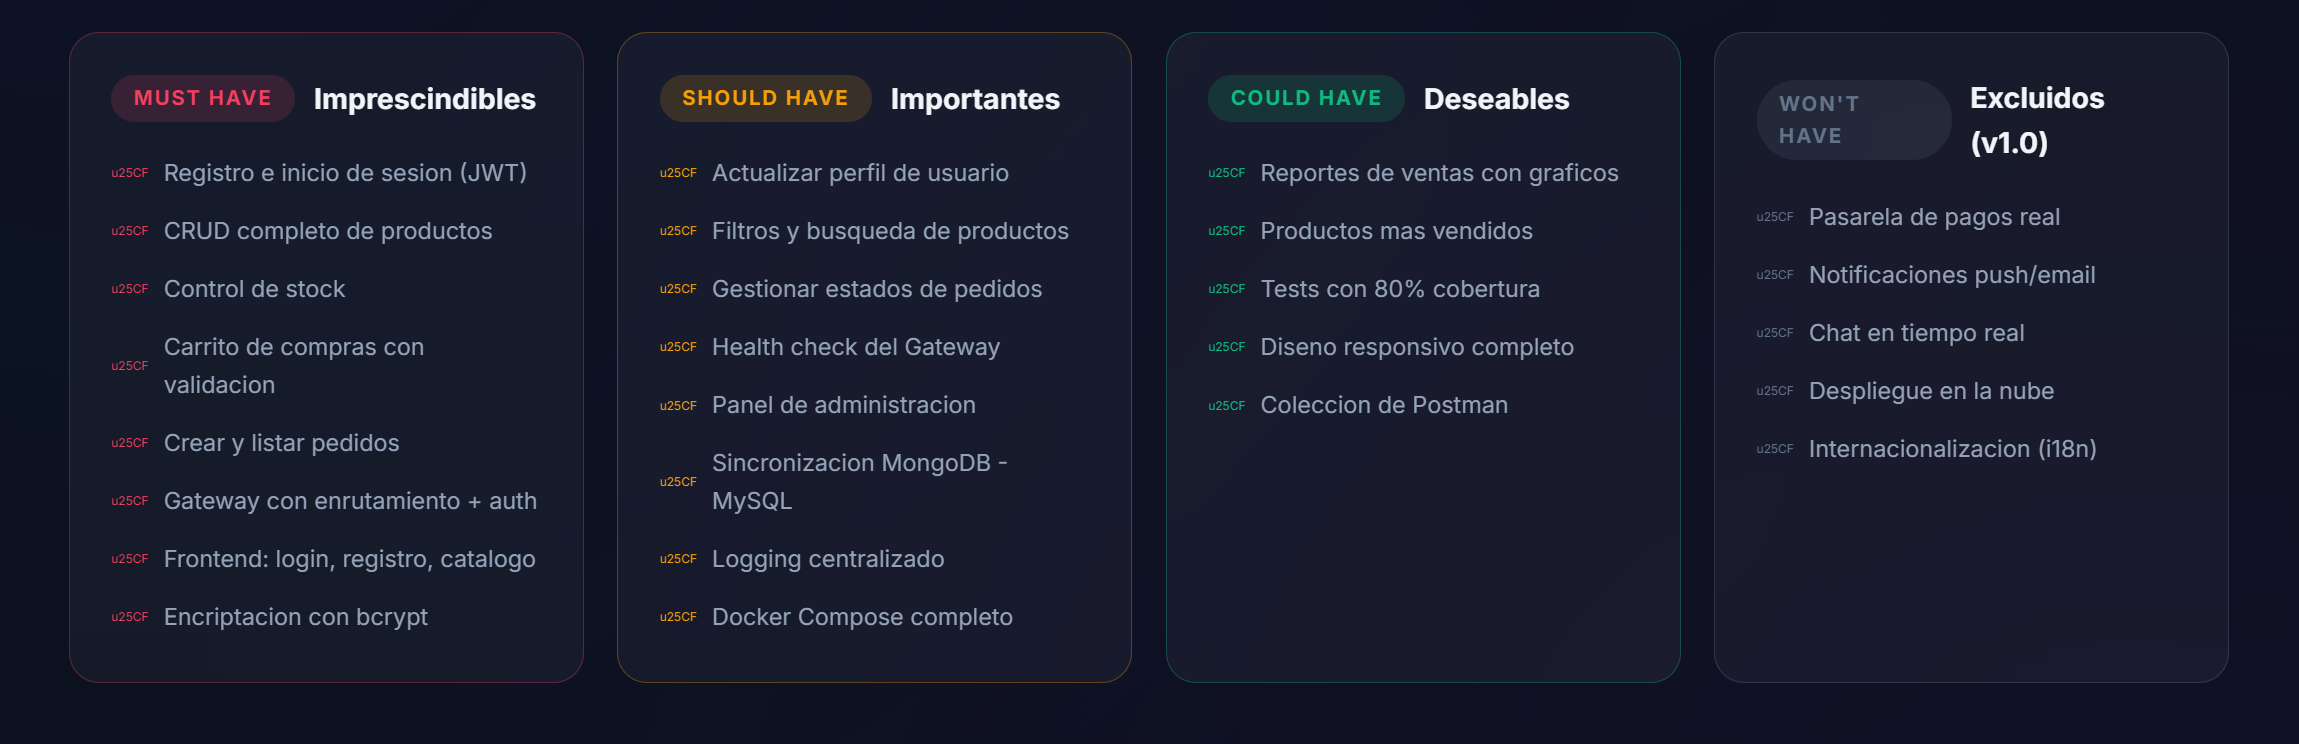
\includegraphics[width=0.85\textwidth]{diagrama_moscow.png}
\caption{Priorizaci\'on MoSCoW de Requisitos}
\label{fig:moscow}
\end{figure}

\subsection{Must Have (Imprescindibles)}
RF-U01--U03, RF-U07--U08, RF-P01--P04, RF-P08, RF-C01--C04, RF-C06--C07, RF-O01--O03, RF-O06--O08, RF-G01--G02, RF-F01--F06, RNF-04--RNF-08.

\subsection{Should Have (Importantes)}
RF-U04--U05, RF-P05--P07, RF-C05, RF-O04--O05, RF-R05, RF-G03, RF-F07--F08, RNF-01--RNF-03, RNF-12--RNF-13.

\subsection{Could Have (Deseables)}
RF-R01--R03, RF-F09, RNF-09--RNF-10, RNF-15--RNF-18.

\subsection{Won't Have (No en esta versi\'on)}
Pasarela de pagos real, notificaciones push/email, chat en tiempo real, despliegue en la nube, internacionalizaci\'on.

\newpage
% ==================== 7. CASOS DE USO ====================
\section{Casos de Uso}

% --- DIAGRAMA: CU-01 ---
\subsection{CU-01: Registrar Usuario}
\begin{figure}[H]
\centering
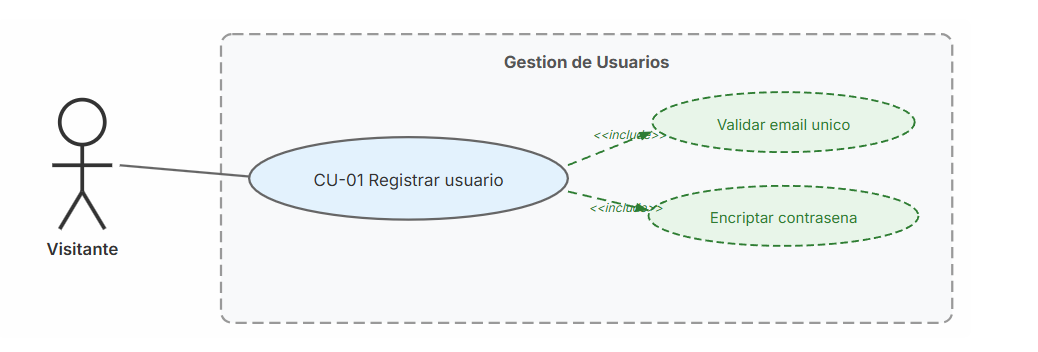
\includegraphics[width=0.85\textwidth]{cu01_registrar_usuario.png}
\caption{Diagrama de Caso de Uso -- CU-01 Registrar Usuario}
\label{fig:cu01}
\end{figure}
\begin{table}[H]
\centering
\begin{tabularx}{\textwidth}{lX}
\toprule
\textbf{Actor} & Visitante \\
\textbf{Precondici\'on} & No posee cuenta en el sistema \\
\textbf{RF asociados} & RF-U01, RF-U07, RF-U08 \\
\textbf{Include} & Validar email \'unico, Encriptar contrase\~na \\
\textbf{Flujo principal} & 1. Accede al formulario de registro \newline 2. Ingresa nombre, email, contrase\~na, tel\'efono \newline 3. Valida email \'unico $\ll$include$\gg$ \newline 4. Encripta contrase\~na $\ll$include$\gg$ \newline 5. Crea cuenta y redirige al login \\
\textbf{Flujo alternativo} & 3a. Email duplicado: muestra error \\
\textbf{Postcondici\'on} & Usuario almacenado en MongoDB \\
\bottomrule
\end{tabularx}
\end{table}

% --- DIAGRAMA: CU-02 ---
\subsection{CU-02: Iniciar Sesi\'on}
\begin{figure}[H]
\centering
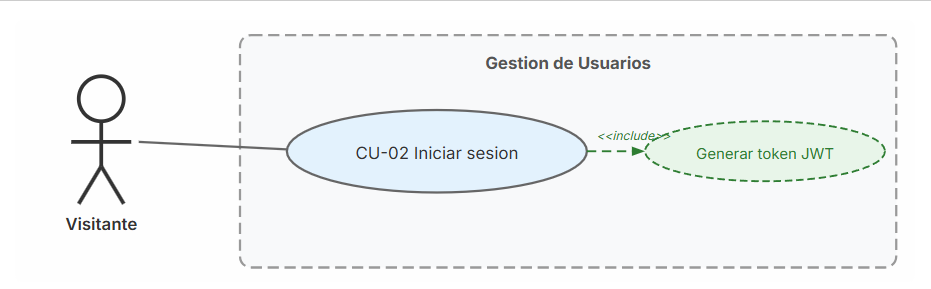
\includegraphics[width=0.85\textwidth]{cu02_iniciar_sesion.png}
\caption{Diagrama de Caso de Uso -- CU-02 Iniciar Sesi\'on}
\label{fig:cu02}
\end{figure}
\begin{table}[H]
\centering
\begin{tabularx}{\textwidth}{lX}
\toprule
\textbf{Actor} & Visitante \\
\textbf{RF asociados} & RF-U02, RF-U08 \\
\textbf{Include} & Generar token JWT \\
\textbf{Flujo principal} & 1. Ingresa email y contrase\~na \newline 2. Verifica credenciales \newline 3. Genera JWT $\ll$include$\gg$ \newline 4. Redirige al home autenticado \\
\textbf{Flujo alternativo} & 2a. Credenciales inv\'alidas: error \\
\textbf{Postcondici\'on} & Token JWT almacenado en el cliente \\
\bottomrule
\end{tabularx}
\end{table}

% --- DIAGRAMA: CU-03 ---
\subsection{CU-03: Gestionar Perfil}
\begin{figure}[H]
\centering
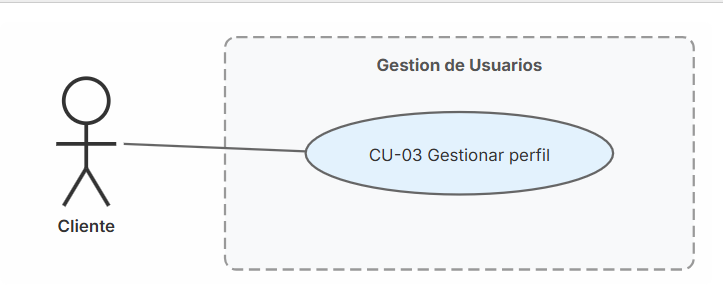
\includegraphics[width=0.85\textwidth]{cu03_gestionar_perfil.png}
\caption{Diagrama de Caso de Uso -- CU-03 Gestionar Perfil}
\label{fig:cu03}
\end{figure}
\begin{table}[H]
\centering
\begin{tabularx}{\textwidth}{lX}
\toprule
\textbf{Actor} & Cliente (autenticado) \\
\textbf{RF asociados} & RF-U03, RF-U04 \\
\textbf{Flujo principal} & 1. Accede a Mi Perfil \newline 2. Visualiza datos actuales \newline 3. Modifica nombre, tel\'efono, direcci\'on \newline 4. Sistema valida y guarda cambios \\
\textbf{Flujo alternativo} & 4a. Datos inv\'alidos: muestra error \\
\bottomrule
\end{tabularx}
\end{table}

% --- DIAGRAMA: CU-04 ---
\subsection{CU-04: Explorar Cat\'alogo}
\begin{figure}[H]
\centering
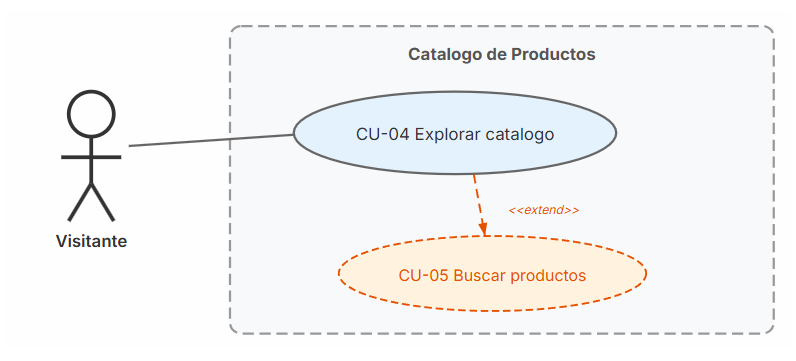
\includegraphics[width=0.85\textwidth]{cu04_explorar_catalogo.png}
\caption{Diagrama de Caso de Uso -- CU-04 Explorar Cat\'alogo}
\label{fig:cu04}
\end{figure}
\begin{table}[H]
\centering
\begin{tabularx}{\textwidth}{lX}
\toprule
\textbf{Actor} & Visitante / Cliente \\
\textbf{RF asociados} & RF-P01, RF-P06 \\
\textbf{Extend} & CU-05 Buscar productos \\
\textbf{Flujo principal} & 1. Accede al cat\'alogo \newline 2. Visualiza grid paginado \newline 3. Filtra por categor\'ia \\
\bottomrule
\end{tabularx}
\end{table}

% --- DIAGRAMA: CU-05 ---
\subsection{CU-05: Buscar Productos}
\begin{figure}[H]
\centering
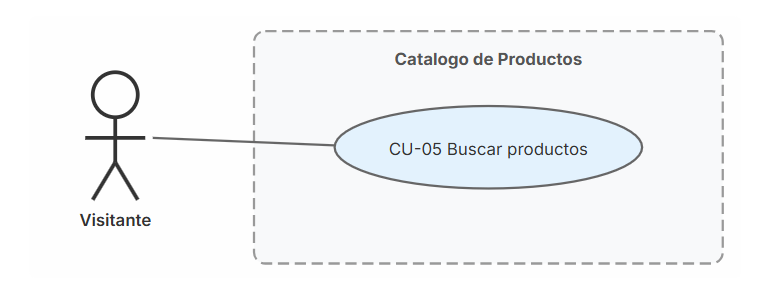
\includegraphics[width=0.85\textwidth]{cu05_buscar_productos.png}
\caption{Diagrama de Caso de Uso -- CU-05 Buscar Productos}
\label{fig:cu05}
\end{figure}
\begin{table}[H]
\centering
\begin{tabularx}{\textwidth}{lX}
\toprule
\textbf{Actor} & Visitante / Cliente \\
\textbf{RF asociados} & RF-P02 \\
\textbf{Flujo principal} & 1. Ingresa t\'ermino en barra de b\'usqueda \newline 2. Sistema busca por nombre/descripci\'on \newline 3. Muestra resultados filtrados \\
\textbf{Flujo alternativo} & 3a. Sin resultados: mensaje informativo \\
\bottomrule
\end{tabularx}
\end{table}

% --- DIAGRAMA: CU-06 ---
\subsection{CU-06: Ver Detalle de Producto}
\begin{figure}[H]
\centering
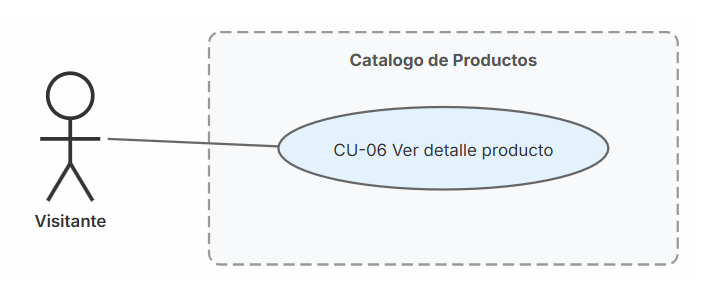
\includegraphics[width=0.85\textwidth]{cu06_detalle_producto.png}
\caption{Diagrama de Caso de Uso -- CU-06 Ver Detalle de Producto}
\label{fig:cu06}
\end{figure}
\begin{table}[H]
\centering
\begin{tabularx}{\textwidth}{lX}
\toprule
\textbf{Actor} & Visitante / Cliente \\
\textbf{RF asociados} & RF-P07 \\
\textbf{Flujo principal} & 1. Selecciona producto del cat\'alogo \newline 2. Muestra nombre, precio, descripci\'on, stock, im\'agenes \newline 3. Opci\'on de agregar al carrito (si Cliente) \\
\bottomrule
\end{tabularx}
\end{table}

% --- DIAGRAMA: CU-07 ---
\subsection{CU-07: Agregar al Carrito}
\begin{figure}[H]
\centering
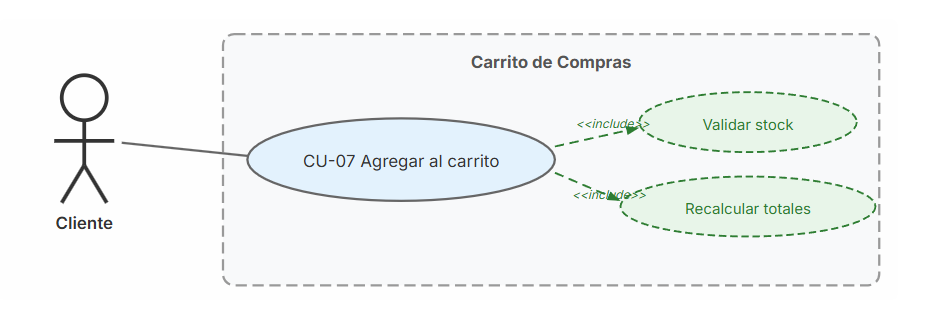
\includegraphics[width=0.85\textwidth]{cu07_agregar_carrito.png}
\caption{Diagrama de Caso de Uso -- CU-07 Agregar al Carrito}
\label{fig:cu07}
\end{figure}
\begin{table}[H]
\centering
\begin{tabularx}{\textwidth}{lX}
\toprule
\textbf{Actor} & Cliente \\
\textbf{RF asociados} & RF-C02, RF-C06, RF-C07 \\
\textbf{Include} & Validar stock, Recalcular totales \\
\textbf{Flujo principal} & 1. Selecciona cantidad \newline 2. Presiona Agregar \newline 3. Valida stock $\ll$include$\gg$ \newline 4. Agrega y recalcula $\ll$include$\gg$ \\
\textbf{Flujo alternativo} & 3a. Sin stock: muestra error \\
\bottomrule
\end{tabularx}
\end{table}

% --- DIAGRAMA: CU-08 ---
\subsection{CU-08: Modificar Carrito}
\begin{figure}[H]
\centering
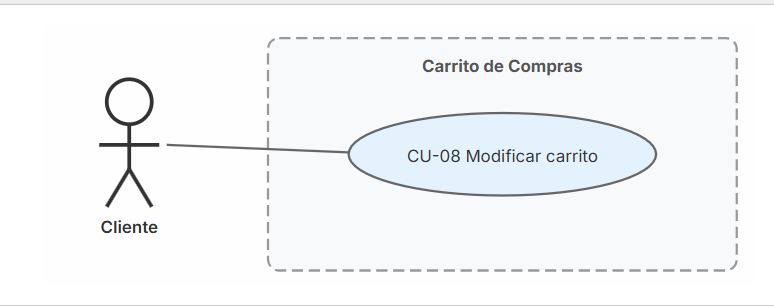
\includegraphics[width=0.85\textwidth]{cu08_modificar_carrito.png}
\caption{Diagrama de Caso de Uso -- CU-08 Modificar Carrito}
\label{fig:cu08}
\end{figure}
\begin{table}[H]
\centering
\begin{tabularx}{\textwidth}{lX}
\toprule
\textbf{Actor} & Cliente \\
\textbf{RF asociados} & RF-C03, RF-C04 \\
\textbf{Flujo principal} & 1. Accede al carrito \newline 2. Cambia cantidad o elimina item \newline 3. Recalcula subtotales y total \\
\bottomrule
\end{tabularx}
\end{table}

% --- DIAGRAMA: CU-09 ---
\subsection{CU-09: Vaciar Carrito}
\begin{figure}[H]
\centering
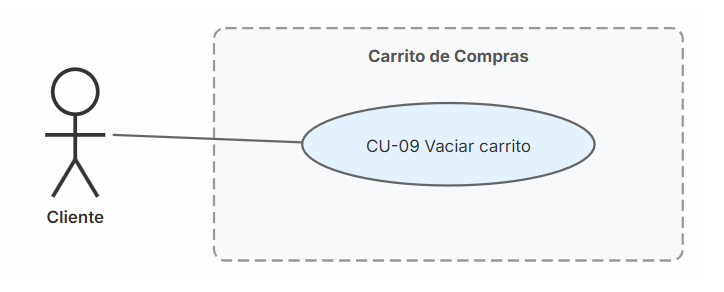
\includegraphics[width=0.85\textwidth]{cu09_vaciar_carrito.png}
\caption{Diagrama de Caso de Uso -- CU-09 Vaciar Carrito}
\label{fig:cu09}
\end{figure}
\begin{table}[H]
\centering
\begin{tabularx}{\textwidth}{lX}
\toprule
\textbf{Actor} & Cliente \\
\textbf{RF asociados} & RF-C05 \\
\textbf{Flujo principal} & 1. Presiona Vaciar carrito \newline 2. Confirma acci\'on \newline 3. Elimina todos los items \\
\bottomrule
\end{tabularx}
\end{table}

% --- DIAGRAMA: CU-10 ---
\subsection{CU-10: Realizar Pedido}
\begin{figure}[H]
\centering
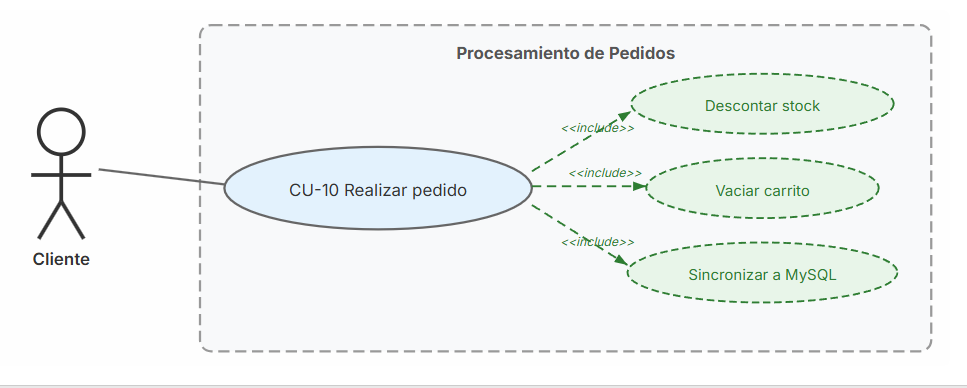
\includegraphics[width=0.85\textwidth]{cu10_realizar_pedido.png}
\caption{Diagrama de Caso de Uso -- CU-10 Realizar Pedido}
\label{fig:cu10}
\end{figure}
\begin{table}[H]
\centering
\begin{tabularx}{\textwidth}{lX}
\toprule
\textbf{Actor} & Cliente \\
\textbf{RF asociados} & RF-O01, RF-O06, RF-O07, RF-O08 \\
\textbf{Include} & Descontar stock, Vaciar carrito, Sincronizar a MySQL \\
\textbf{Flujo principal} & 1. Confirma direcci\'on y pago \newline 2. Genera n\'umero de orden \'unico \newline 3. Descuenta stock $\ll$include$\gg$ \newline 4. Vac\'ia carrito $\ll$include$\gg$ \newline 5. Sincroniza a MySQL $\ll$include$\gg$ \\
\textbf{Flujo alternativo} & 3a. Fallo stock: rollback \\
\textbf{Postcondici\'on} & Pedido creado, stock actualizado, carrito vac\'io \\
\bottomrule
\end{tabularx}
\end{table}

% --- DIAGRAMA: CU-11 ---
\subsection{CU-11: Consultar Pedidos}
\begin{figure}[H]
\centering
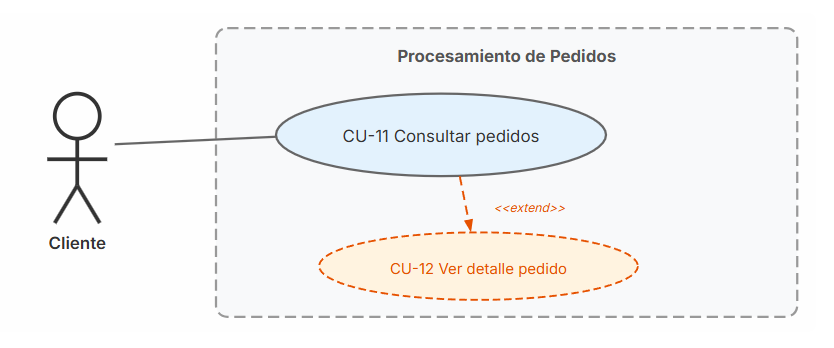
\includegraphics[width=0.85\textwidth]{cu11_consultar_pedidos.png}
\caption{Diagrama de Caso de Uso -- CU-11 Consultar Pedidos}
\label{fig:cu11}
\end{figure}
\begin{table}[H]
\centering
\begin{tabularx}{\textwidth}{lX}
\toprule
\textbf{Actor} & Cliente \\
\textbf{RF asociados} & RF-O02, RF-O03 \\
\textbf{Extend} & CU-12 Ver detalle de pedido \\
\textbf{Flujo principal} & 1. Lista pedidos con fecha, monto, estado \newline 2. Selecciona pedido para detalle $\ll$extend$\gg$ \\
\bottomrule
\end{tabularx}
\end{table}

% --- DIAGRAMA: CU-12 ---
\subsection{CU-12: Ver Detalle de Pedido}
\begin{figure}[H]
\centering
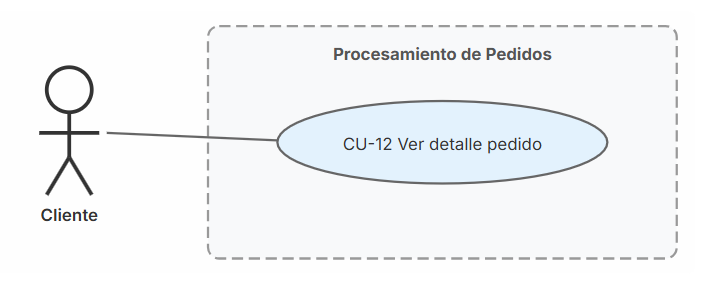
\includegraphics[width=0.85\textwidth]{cu12_detalle_pedido.png}
\caption{Diagrama de Caso de Uso -- CU-12 Ver Detalle de Pedido}
\label{fig:cu12}
\end{figure}
\begin{table}[H]
\centering
\begin{tabularx}{\textwidth}{lX}
\toprule
\textbf{Actor} & Cliente \\
\textbf{RF asociados} & RF-O03 \\
\textbf{Flujo principal} & 1. Selecciona pedido de la lista \newline 2. Muestra items, cantidades, precios, estado \newline 3. Historial de cambios de estado \\
\bottomrule
\end{tabularx}
\end{table}

% --- DIAGRAMA: CU-13 ---
\subsection{CU-13: Gestionar Productos (Admin)}
\begin{figure}[H]
\centering
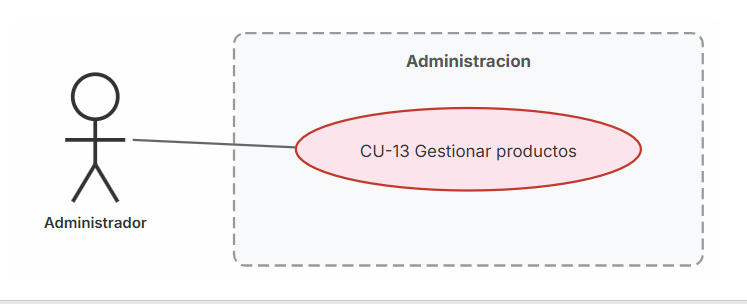
\includegraphics[width=0.85\textwidth]{cu13_gestionar_productos.png}
\caption{Diagrama de Caso de Uso -- CU-13 Gestionar Productos}
\label{fig:cu13}
\end{figure}
\begin{table}[H]
\centering
\begin{tabularx}{\textwidth}{lX}
\toprule
\textbf{Actor} & Administrador \\
\textbf{RF asociados} & RF-P03, RF-P04, RF-P05, RF-P08 \\
\textbf{Flujo principal} & 1. CRUD completo de productos \newline 2. Gestiona stock y estado activo/inactivo \newline 3. Sube im\'agenes del producto \\
\bottomrule
\end{tabularx}
\end{table}

% --- DIAGRAMA: CU-14 ---
\subsection{CU-14: Gestionar Pedidos (Admin)}
\begin{figure}[H]
\centering
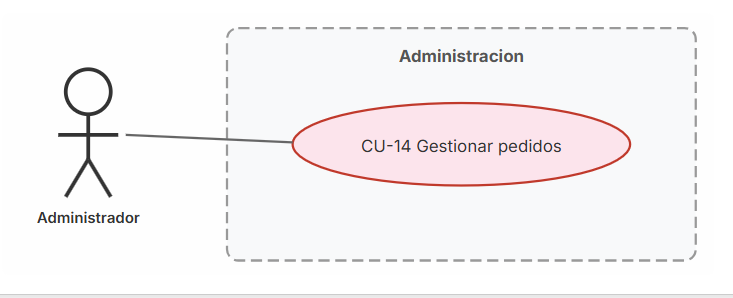
\includegraphics[width=0.85\textwidth]{cu14_gestionar_pedidos.png}
\caption{Diagrama de Caso de Uso -- CU-14 Gestionar Pedidos}
\label{fig:cu14}
\end{figure}
\begin{table}[H]
\centering
\begin{tabularx}{\textwidth}{lX}
\toprule
\textbf{Actor} & Administrador \\
\textbf{RF asociados} & RF-O04, RF-O05 \\
\textbf{Flujo principal} & 1. Ve todos los pedidos del sistema \newline 2. Actualiza estados (pendiente, enviado, entregado) \\
\bottomrule
\end{tabularx}
\end{table}

% --- DIAGRAMA: CU-15 ---
\subsection{CU-15: Gestionar Usuarios (Admin)}
\begin{figure}[H]
\centering
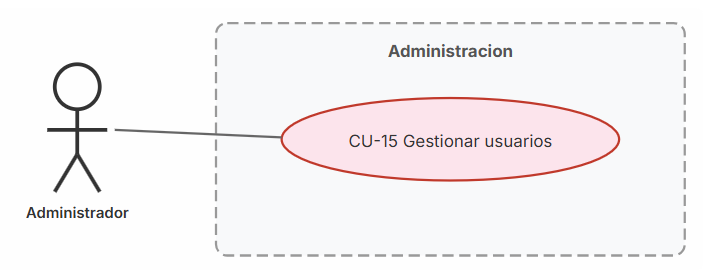
\includegraphics[width=0.85\textwidth]{cu15_gestionar_usuarios.png}
\caption{Diagrama de Caso de Uso -- CU-15 Gestionar Usuarios}
\label{fig:cu15}
\end{figure}
\begin{table}[H]
\centering
\begin{tabularx}{\textwidth}{lX}
\toprule
\textbf{Actor} & Administrador \\
\textbf{RF asociados} & RF-U05, RF-U06 \\
\textbf{Flujo principal} & 1. Lista todos los usuarios \newline 2. Activa/desactiva cuentas \newline 3. Elimina usuarios si es necesario \\
\bottomrule
\end{tabularx}
\end{table}

% --- DIAGRAMA: CU-16 ---
\subsection{CU-16: Consultar Reportes (Admin)}
\begin{figure}[H]
\centering
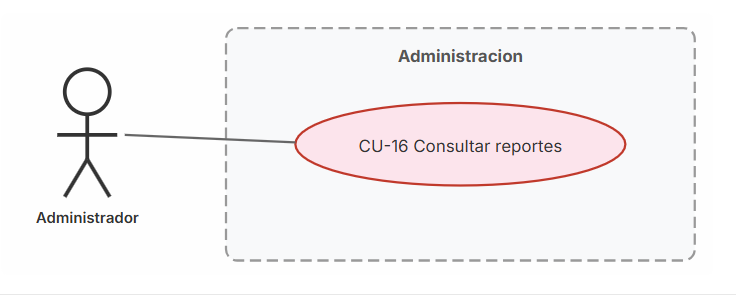
\includegraphics[width=0.85\textwidth]{cu16_consultar_reportes.png}
\caption{Diagrama de Caso de Uso -- CU-16 Consultar Reportes}
\label{fig:cu16}
\end{figure}
\begin{table}[H]
\centering
\begin{tabularx}{\textwidth}{lX}
\toprule
\textbf{Actor} & Administrador \\
\textbf{RF asociados} & RF-R01 a RF-R05 \\
\textbf{Flujo principal} & 1. Selecciona tipo de reporte y rango de fechas \newline 2. Consulta datos en MySQL \newline 3. Muestra gr\'aficos y estad\'isticas \\
\bottomrule
\end{tabularx}
\end{table}

\newpage
% ==================== 8. DIAGRAMAS ADICIONALES ====================
\section{Diagramas Adicionales}

% --- DIAGRAMA: ENTIDADES ---
\begin{figure}[H]
\centering
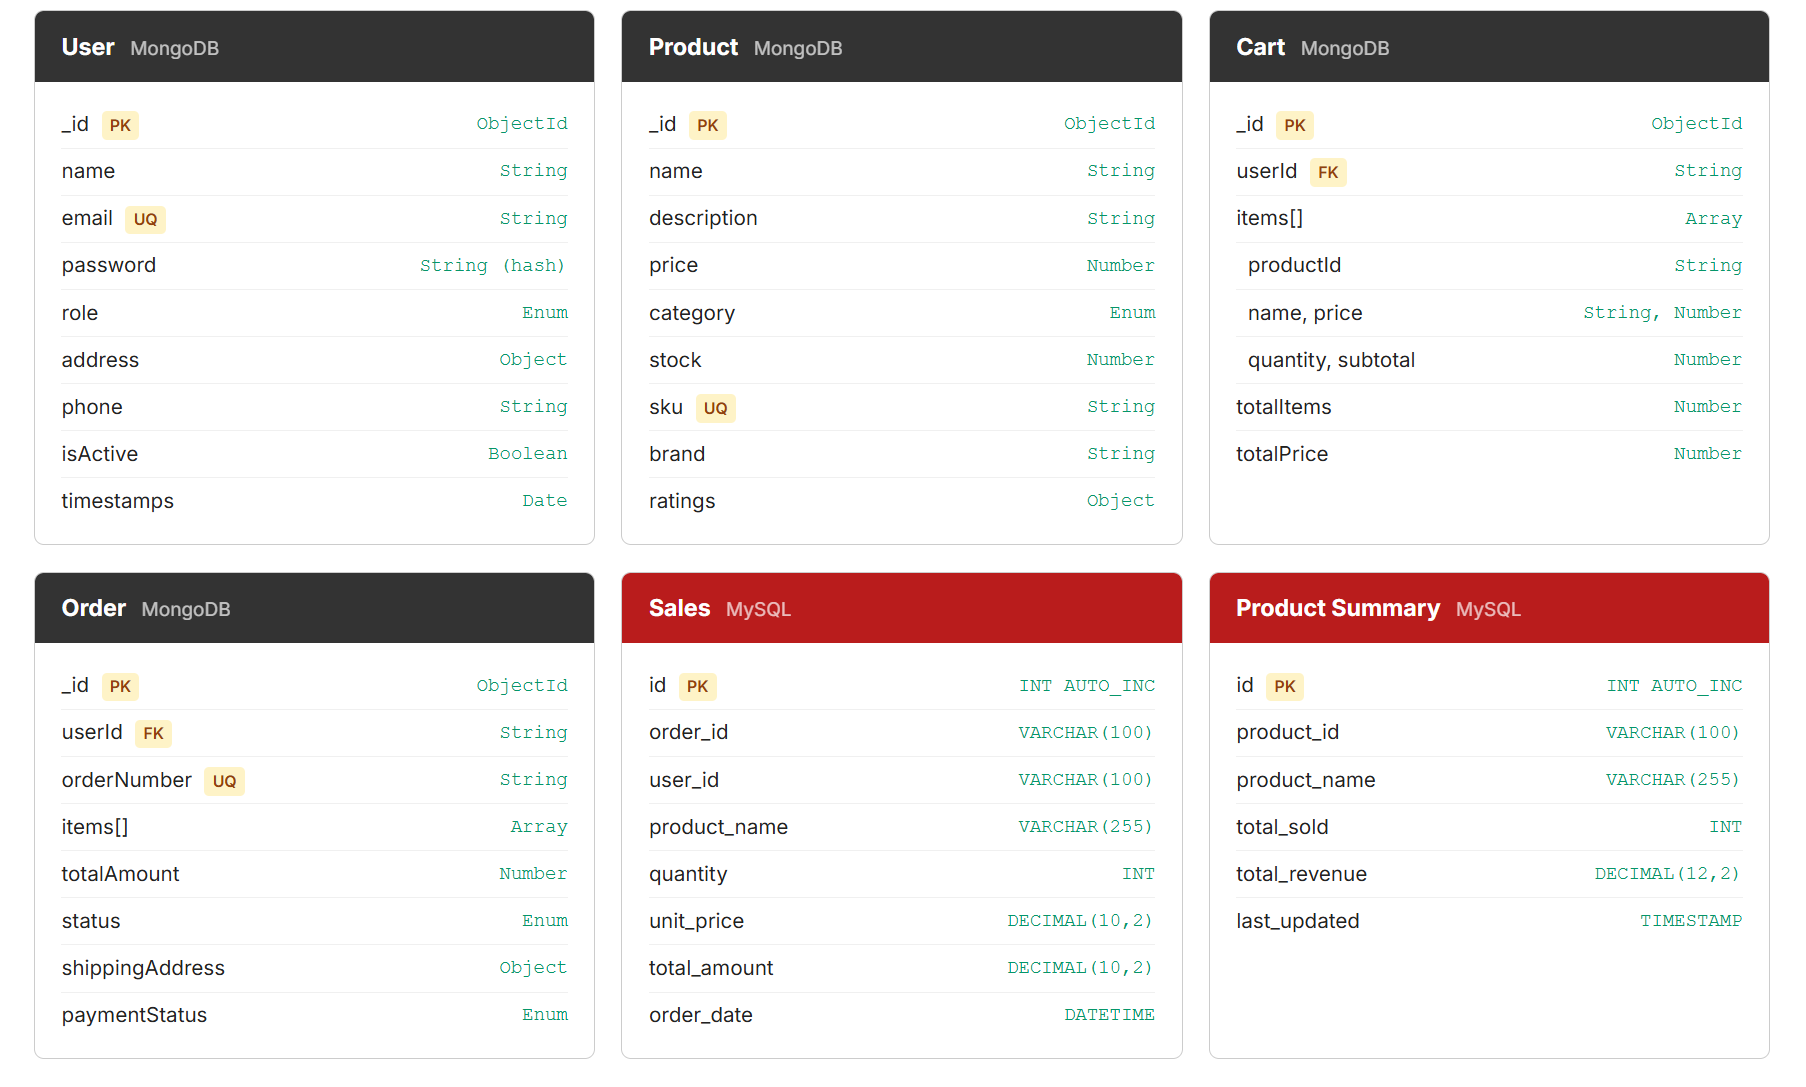
\includegraphics[width=0.85\textwidth]{diagrama_entidades.png}
\caption{Diagrama de Entidades del Sistema}
\label{fig:entidades}
\end{figure}

% --- DIAGRAMA: COMUNICACION ---
\begin{figure}[H]
\centering
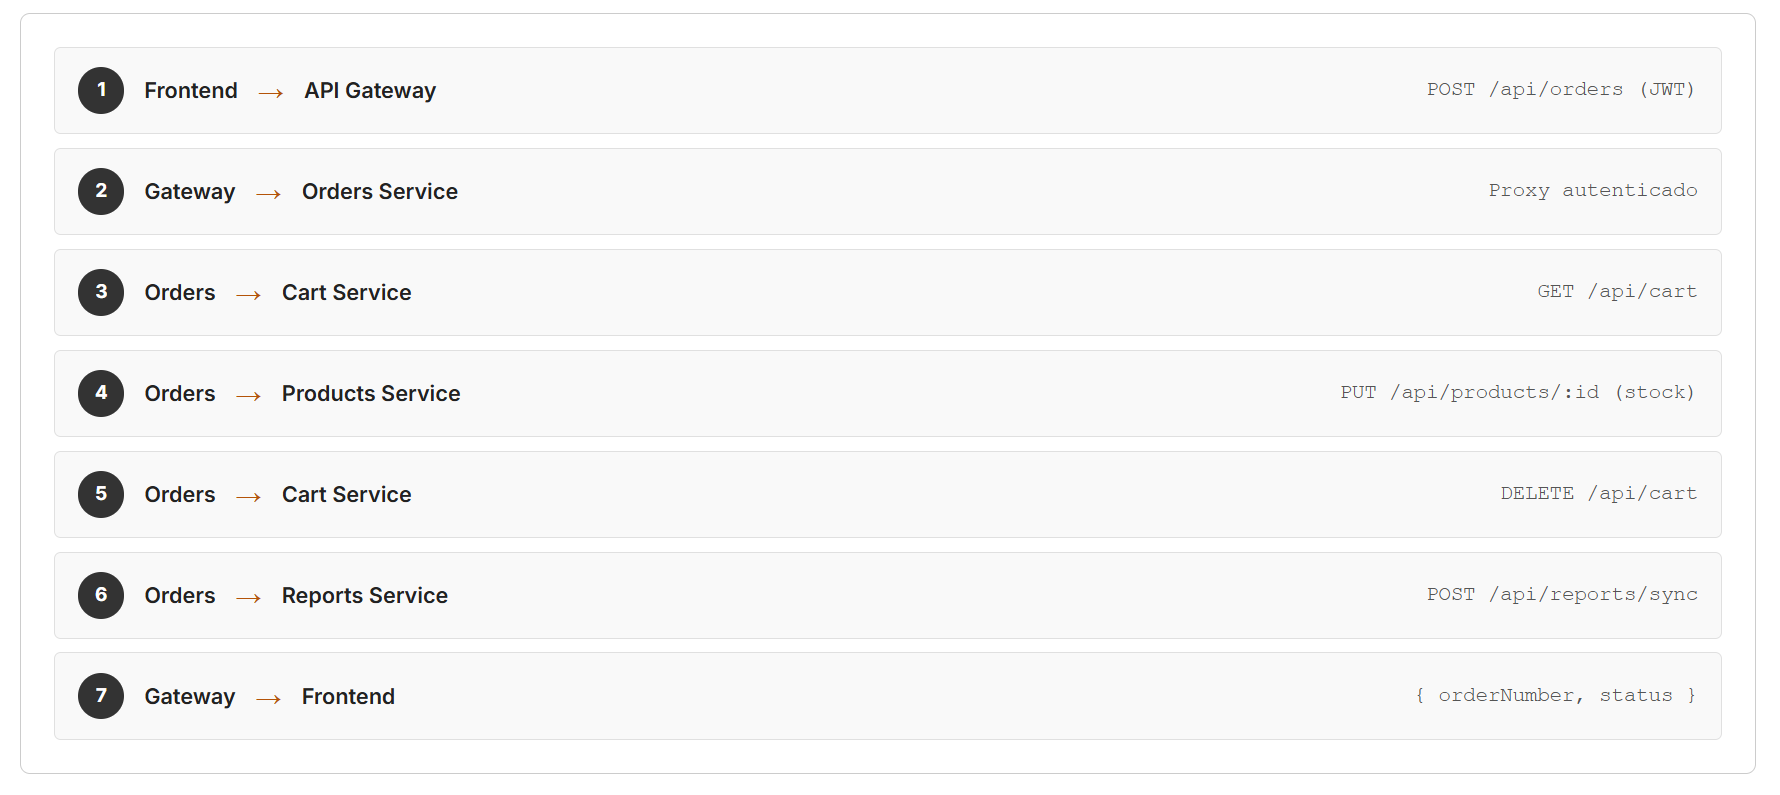
\includegraphics[width=0.85\textwidth]{diagrama_comunicacion.png}
\caption{Flujo de Comunicaci\'on entre Microservicios}
\label{fig:comunicacion}
\end{figure}

% --- TABLA: MATRIZ DE TRAZABILIDAD ---
\begin{longtable}{llllc}
\caption{Matriz de Trazabilidad: RF -- Casos de Uso -- Microservicios} \label{tab:trazabilidad} \\
\toprule
\textbf{RF ID} & \textbf{Requisito} & \textbf{Caso de Uso} & \textbf{Microservicio} & \textbf{Prioridad} \\
\midrule
\endfirsthead
\toprule
\textbf{RF ID} & \textbf{Requisito} & \textbf{Caso de Uso} & \textbf{Microservicio} & \textbf{Prioridad} \\
\midrule
\endhead
\midrule
\multicolumn{5}{r}{\textit{Contin\'ua en la siguiente p\'agina}} \\
\endfoot
\bottomrule
\endlastfoot
RF-U01 & Registro de usuario       & CU-01       & Users Service     & Alta  \\
RF-U02 & Inicio de sesi\'on        & CU-02       & Users Service     & Alta  \\
RF-U03 & Consultar perfil          & CU-02       & Users Service     & Alta  \\
RF-U04 & Actualizar perfil         & CU-02       & Users Service     & Media \\
RF-U05 & Listar usuarios           & CU-06       & Users Service     & Media \\
RF-U06 & Eliminar usuario          & CU-06       & Users Service     & Baja  \\
RF-U07 & Validaci\'on email \'unico & CU-01      & Users Service     & Alta  \\
RF-U08 & Encriptaci\'on contrase\~na & CU-01, CU-02 & Users Service  & Alta  \\
\midrule
RF-P01 & Listar productos          & CU-03       & Products Service  & Alta  \\
RF-P02 & Detalle de producto       & CU-03       & Products Service  & Alta  \\
RF-P03 & Crear producto            & CU-06       & Products Service  & Alta  \\
RF-P04 & Actualizar producto       & CU-06       & Products Service  & Alta  \\
RF-P05 & Eliminar producto         & CU-06       & Products Service  & Media \\
RF-P06 & Filtrar por categor\'ia   & CU-03       & Products Service  & Media \\
RF-P07 & Buscar productos          & CU-03       & Products Service  & Media \\
RF-P08 & Control de stock          & CU-04, CU-05 & Products Service & Alta  \\
\midrule
RF-C01 & Ver carrito               & CU-04       & Cart Service      & Alta  \\
RF-C02 & Agregar al carrito        & CU-04       & Cart Service      & Alta  \\
RF-C03 & Actualizar cantidad       & CU-04       & Cart Service      & Alta  \\
RF-C04 & Eliminar item             & CU-04       & Cart Service      & Alta  \\
RF-C05 & Vaciar carrito            & CU-05       & Cart Service      & Media \\
RF-C06 & Validaci\'on de stock     & CU-04       & Cart + Products   & Alta  \\
RF-C07 & C\'alculo autom\'atico    & CU-04       & Cart Service      & Alta  \\
\midrule
RF-O01 & Crear pedido              & CU-05       & Orders Service    & Alta  \\
RF-O02 & Listar mis pedidos        & CU-05       & Orders Service    & Alta  \\
RF-O03 & Detalle de pedido         & CU-05       & Orders Service    & Alta  \\
RF-O04 & Actualizar estado         & CU-06       & Orders Service    & Alta  \\
RF-O05 & Listar todos los pedidos  & CU-06       & Orders Service    & Media \\
RF-O06 & N\'umero de orden \'unico & CU-05       & Orders Service    & Alta  \\
RF-O07 & Descontar stock           & CU-05       & Orders + Products & Alta  \\
RF-O08 & Vaciar carrito post-pedido & CU-05      & Orders + Cart     & Alta  \\
\midrule
RF-R01 & Reporte de ventas         & CU-07       & Reports Service   & Media \\
RF-R02 & Productos m\'as vendidos  & CU-07       & Reports Service   & Media \\
RF-R03 & Ingresos totales          & CU-07       & Reports Service   & Media \\
RF-R04 & Actividad de usuarios     & CU-07       & Reports Service   & Baja  \\
RF-R05 & Sincronizaci\'on de datos & CU-07       & Reports + Orders  & Alta  \\
\midrule
RF-G01 & Enrutamiento              & Todos       & API Gateway       & Alta  \\
RF-G02 & Auth centralizada         & Todos       & API Gateway       & Alta  \\
RF-G03 & Health check              & N/A         & API Gateway       & Media \\
\end{longtable}

\newpage
% ==================== 9. LIMITACIONES ====================
\section{Limitaciones}

\subsection{Limitaciones T\'ecnicas}
\begin{table}[H]
\centering
\begin{tabularx}{\textwidth}{lX}
\toprule
\textbf{ID} & \textbf{Descripci\'on} \\
\midrule
L-01 & Sin pasarela de pagos real (simulaci\'on) \\
L-02 & Ejecuci\'on local, no en producci\'on en la nube \\
L-03 & Sin notificaciones en tiempo real (WebSockets) \\
L-04 & Im\'agenes manejadas como URLs externas \\
L-05 & MongoDB y MySQL sin r\'eplicas \\
\bottomrule
\end{tabularx}
\end{table}

\subsection{Limitaciones del Alcance}
\begin{table}[H]
\centering
\begin{tabularx}{\textwidth}{lX}
\toprule
\textbf{ID} & \textbf{Descripci\'on} \\
\midrule
L-06 & Un solo idioma (espa\~nol) \\
L-07 & Sin sistema de cupones o descuentos \\
L-08 & Sin c\'alculo de costos de env\'io diferenciados \\
L-09 & Sin reviews/calificaciones de productos \\
L-10 & Sin recuperaci\'on de contrase\~na \\
\bottomrule
\end{tabularx}
\end{table}

\subsection{Limitaciones de Rendimiento}
\begin{table}[H]
\centering
\begin{tabularx}{\textwidth}{lX}
\toprule
\textbf{ID} & \textbf{Descripci\'on} \\
\midrule
L-11 & Comunicaci\'on s\'incrona HTTP, sin colas de mensajes \\
L-12 & Sin cach\'e (Redis) \\
L-13 & Sin CDN para assets est\'aticos \\
\bottomrule
\end{tabularx}
\end{table}

\newpage
% ==================== 10. GLOSARIO ====================
\section{Glosario de T\'erminos}

\begin{longtable}{lp{10cm}}
\toprule
\textbf{T\'ermino} & \textbf{Definici\'on} \\
\midrule
\endhead
API Gateway & Punto de entrada \'unico que redirige peticiones al microservicio correspondiente \\
Autenticaci\'on & Verificaci\'on de identidad mediante credenciales \\
Autorizaci\'on & Verificaci\'on de permisos para una acci\'on espec\'ifica \\
bcrypt & Algoritmo de hashing para encriptar contrase\~nas \\
Checkout & Proceso de confirmaci\'on de compra \\
CORS & Cross-Origin Resource Sharing \\
Docker & Plataforma de contenerizaci\'on \\
Docker Compose & Orquestaci\'on de aplicaciones multi-contenedor \\
Express.js & Framework web minimalista para Node.js \\
JWT & JSON Web Token para autenticaci\'on stateless \\
Microservicio & M\'odulo independiente con su propia base de datos \\
MongoDB & Base de datos NoSQL orientada a documentos \\
Mongoose & ODM para MongoDB en Node.js \\
MySQL & Sistema de gesti\'on de BD relacional \\
Node.js & Entorno de ejecuci\'on JavaScript del servidor \\
Pinia & Gesti\'on de estado global para Vue.js \\
REST & Estilo arquitect\'onico para APIs web \\
Rollback & Reversi\'on de operaci\'on ante fallo \\
Sequelize & ORM para bases de datos SQL en Node.js \\
SPA & Single Page Application \\
Vite & Herramienta de build frontend r\'apida \\
Vue.js & Framework progresivo de JavaScript para UI \\
Winston & Librer\'ia de logging para Node.js \\
\bottomrule
\end{longtable}

\vfill
\begin{center}
\rule{0.5\textwidth}{0.4pt}\\[6pt]
{\small Documento generado como parte del proyecto \textbf{NexaCommerce}}\\
{\small Universidad de las Fuerzas Armadas -- ESPE, 2023}
\end{center}

\end{document}
